%
% Niniejszy plik stanowi przykład formatowania pracy magisterskiej na
% Wydziale MIM UW.  Szkielet użytych poleceń można wykorzystywać do
% woli, np. formatujac wlasna prace.
%
% Zawartosc merytoryczna stanowi oryginalnosiagniecie
% naukowosciowe Marcina Wolinskiego.  Wszelkie prawa zastrzeżone.
%
% Copyright (c) 2001 by Marcin Woliński <M.Wolinski@gust.org.pl>
% Poprawki spowodowane zmianami przepisów - Marcin Szczuka, 1.10.2004
% Poprawki spowodowane zmianami przepisow i ujednolicenie 
% - Seweryn Karłowicz, 05.05.2006
% Dodanie wielu autorów i tłumaczenia na angielski - Kuba Pochrybniak, 29.11.2016

% dodaj opcję [licencjacka] dla pracy licencjackiej
% dodaj opcję [en] dla wersji angielskiej (mogą być obie: [licencjacka,en])
\makeatletter
\newenvironment{mcases}[1][l]
 {\let\@ifnextchar\new@ifnextchar
  \left\lbrace
  \def\arraystretch{1.2}%
  \array{@{}l@{\quad}#1@{}}}
 {\endarray\right.}
\makeatother

\documentclass[licencjacka]{pracamgr}
\usepackage[polish]{babel}
\usepackage{graphicx}
\usepackage{caption}
\usepackage{float}
\usepackage{subcaption}
\usepackage{amsmath}
\usepackage{algorithm2e}


% Dane magistranta:
\autor{Aleksander Mućk}{382184}


% Dane magistrantów:
%\autor{Aleksander Mućk}{342007}

\title{Algorytmy do klastrowania duplikacji genomowych}


\tytulang{Algorithms for the clustering of genomic duplication}

%kierunek: 
% - matematyka, informacyka, ...
% - Mathematics, Computer Science, ...
\kierunek{Bioinformatyka i Biologia Systemów}

% informatyka - nie okreslamy zakresu (opcja zakomentowana)
% matematyka - zakres moze pozostac nieokreslony,
% a jesli ma byc okreslony dla pracy mgr,
% to przyjmuje jedna z wartosci:
% {metod matematycznych w finansach}
% {metod matematycznych w ubezpieczeniach}
% {matematyki stosowanej}
% {nauczania matematyki}
% Dla pracy licencjackiej mamy natomiast
% mozliwosc wpisania takiej wartosci zakresu:
% {Jednoczesnych Studiow Ekonomiczno--Matematycznych}

% \zakres{Tu wpisac, jesli trzeba, jedna z opcji podanych wyzej}

% Praca wykonana pod kierunkiem:
% (podać tytuł/stopień imię i nazwisko opiekuna
% Instytut
% ew. Wydział ew. Uczelnia (jeżeli nie MIM UW))
\opiekun{dra hab. Pawła Góreckiego\\
  }

% miesiąc i~rok:
\date{Sierpień 2019}

%Podać dziedzinę wg klasyfikacji Socrates-Erasmus:
\dziedzina{ 
%11.0 Matematyka, Informatyka:\\ 
%11.1 Matematyka\\ 
%11.2 Statystyka\\ 
%11.3 Informatyka\\ 
%11.4 Sztuczna inteligencja\\ 
%11.5 Nauki aktuarialne\\
11.9 Inne nauki matematyczne i informatyczne
}

%Klasyfikacja tematyczna wedlug AMS (matematyka) lub ACM (informatyka)
\klasyfikacja{Computional biology, Applied computing, Life and medical sciences}

% Słowa kluczowe:
\keywords{duplikacja genu, drzewo genów, drzewo gatunków, analiza filogenetyczna, drzewo uzgadniające, Python, scenariusz ewolucyjny, strata genu, minimalizacja kosztu ewolucyjnego}

% Tu jest dobre miejsce na Twoje własne makra i~środowiska:
\newtheorem{defi}{Definicja}[section]

% koniec definicji

\begin{document}

\maketitle

%tu idzie streszczenie na strone poczatkowa

\begin{abstract}
   Niniejsza praca przedstawia propozycje rozwiązań algorytmicznych dla problemów klastrowania duplikacji genomowych w oparciu o scenariusze ewolucyjne. W części pierwszej wprowadzane są podstawowe pojęcia dotyczące drzew genów, gatunków, modeli ich uzgadniania oraz tworzenia scenariuszy ewolucyjnych. Omówiony został również problem przeliczania i klastrowania duplikacji genomowych. W części drugiej opisana została proponowana heurystyka wraz z przykładowymi testami oraz jej implementacją w języku Python.
\end{abstract}


\renewcommand{\contentsname}{Spis Treści}
\tableofcontents
%\listoffigures
%\listoftables

\chapter*{Wprowadzenie}
\addcontentsline{toc}{chapter}{Wprowadzenie}


Badanie drzew genów i gatunków, a w szczególności zależności między nimi może odpowiedzieć na pytania w jaki sposób wyodrębniały się gatunki przez pryzmat zmian w ich genomie. Mimo wszystko jednak należy pamiętać, że pokrewieństwo gatunków nie zawsze implikuje pokrewieństwo genów. W szczególności drzewo ewolucyjne genów nie musi pokrywać się z odpowiadającym im drzewem gatunków, które samo w sobie nie jest tak bardzo bardzo zróżnicowane jak drzewo genów. Tworzenie scenariuszy ewolucyjnych dzięki którym możemy poznać w jaki sposób ewolucja genów wpływała na ewolucję gatunków jest zadaniem nietrywialnym. Potrzebne są narzędzia, które potrafiłyby ocenić scenariusze pod kątem ilości zdarzeń ewolucyjnych i przyporządkować je we właściwe miejsca historii ewolucyjnej.

Należy zaznaczyć, że wybranie właściwego scenariusza ewolucyjnego nie jest zadaniem łatwym, ponieważ takich scenariuszy, wyjaśniających ewolucję danej rodziny genów, może być nieskończenie wiele. Problem jeszcze bardziej komplikuje się gdy w badaniach uwzględnimy wiele drzew genów.

W niniejszej pracy proponowane są algorytm, które oceniają zbiór scenariuszy tworząc na ich podstawie jeden, którego koszt, liczony jako ilość duplikacji, będzie możliwie najmniejszy.
\\
Praca składa się z~czterech rozdziałów i~dodatków.
W~rozdziale \ref{r:pojecia} przedstawiono podstawowe pojęcia dotyczące drzew genów, drzew gatunków oraz modeli i scenariuszy ewolucyjnych.  
Rozdział~\ref{r:heurystyka} przedstawia propozycję heurystyki wraz~z jej testami na rzeczywistych danych.  W~rozdziale tym opisano również implementację i sposób użycia programu napisanego na podstawie przybliżonej we wcześniejszej sekcji heurystyki.
Ostatni rozdział zawiera przemyślenia dotyczące możliwego użycia algorytmu i perspektyw jego rozwoju. W~dodatkach umieszczono fragmenty kodu, przykładowe dane wejściowe i~wyniki działania algorytmu.

\chapter{Podstawowe pojęcia}\label{r:pojecia}

W tym rozdziale poruszane są pojęcia i definicje niezbędne do zrozumienia problematyki klastrowania duplikacji genomowych. 
\section{Wstęp biologiczny}

Ewolucja biologiczna jest procesem zmian w trakcie których organizmy stopniowo nabywają lub tracą pewne cechy. Jest to element kluczowy dla powstawania nowych gatunków: specjacji. Śledzenie w jaki sposób kształtowały się nowe gatunki i w jaki sposób zachodziły na Ziemi procesy ewolucyjne jest zadaniem złożonym i wymagającym specyficznego podejścia. Jednym z możliwych sposobów przedstawienia historii ewolucyjnej gatunków jest drzewo filogenetyczne, które przedstawiają zależności ewolucyjne pomiędzy umieszczonymi na nim gatunkami lub genami. 

Początkowo za wyznacznik pokrewieństwa gatunków służyło podobieństwo morfologiczne, jednak obecnie często stosuje się metody polegające na badaniu podobieństwa danych rodzin genów. Można założyć, że im większe podobieństwo genów danych organizmów tym bliżej są one spokrewnione. Z punktu widzenia tej pracy genom jest niczym więcej jak zbiorem genów obecnym w danym organizmie. 


\section{Drzewa genów i gatunków}

W pracy tej drzewo to ukorzenione, binarne drzewo T o zbiorze krawędzi skierowanych $E_T$~i zbiorze węzłów~$V_T$:
\begin{center}
T = <$V_T$ , $E_T$>.
\end{center}
%($v_1$ , $v_2$) takie, że $V_T$ \ni $v_x$ , $v_y$ .
gdzie $E_T$ zawiera pary węzłów ($V$,$W$) takie, że $V$,$W$ $\in$ $V_T$. Węzły z których nie wychodzą żadne krawędzie nazywane są liśćmi, a korzeń jest węzłem do którego nie prowadzą żadne krawędzie (nieposiadającym rodzica). Węzeł $V$ jest przodkiem węzła $W$ jeśli istnieje ścieżka skierowana z węzła $V$ do węzła $W$. Liczba krawędzi w ścieżce od węzła $V$ do węzła $W$ jest nazywana długością. Poddrzewem węzła $V$ jest drzewo oznaczone $T(V)$ w którym węzeł $V$ jest korzeniem. 
%Wszystkie etykiety obecne na liściach widoczne z wierzchołka $v_x$ oznaczmy jako L($v_x$).

Związki między gatunkami przedstawia się za pomocą drzewa~T, zwanego drzewem gatunków~S.
\begin{defi}\label{Drzewa gatunków}
  Drzewo gatunków to takie drzewo S, gdzie każdy liść reprezentuje gatunek, a~węzły wewnętrzne nazywamy specjacjami. Zbiór wszystkich gatunków (liści) oznaczony jest jako $L(S)$. 
\end{defi}

Związki między genami w danej rodzinie przedstawia się za pomocą drzewa~T, zwanego drzewem genów~G.
\begin{defi}\label{Drzewa genów}
  Drzewo genów to takie drzewo G, gdzie każdy liść reprezentuje gen i jest etykietowony gatunkiem, z którego dany gen został zsekwencjonowany. Zbiór wszystkich gatunków (etykiet) oznaczony jest jako $L(G)$.
\end{defi}


\begin{figure}[H]
	\centering
	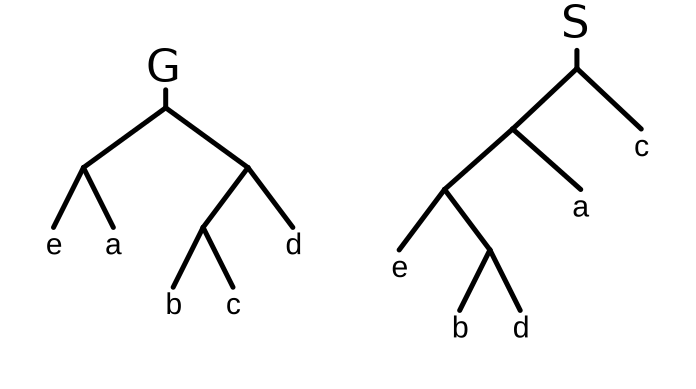
\includegraphics[width=100mm]{./pictures/spec_gen.png}
	\caption{Przykładowe drzewa genów G i gatunków S.}
\end{figure}

\section{Uzgodnienie drzew}
Bardzo częste różnice struktury drzewa genów w stosunku do historii ewolucyjnej opisanej drzewem gatunków wymagają mapowania węzłów drzewa G na węzły znajdujące się w drzewie S. Jest to krok niezbędny by zrozumieć w jaki sposób ewolucja gatunków wpływała na strukturę ich genomów. 

\subsection{Mapowanie LCA}
Podstawowym algorytmem dla tego typu uzgodnień jest \textbf{algorytm LCA} (ang. \textit{Lowest Common Ancestor}; pl. \textit{Najniższy Wspólny Przodek}) \cite{lca}. Najniższym przodkiem węzłów $V$ i $X$ to taki węzeł oznaczony jako $LCA(V,W)$, który jest przodkiem obu węzłów i którego długość ścieżki od korzenia drzewa jest największa. Najniższego wspólnego przodka dwóch węzłów można policzyć w czasie stały po liniowym, jednorazowym preprocesingu. 

\begin{defi}
Dla drzewa genów G i drzewa gatunków S takich, że $L(G)$ $\subseteq$ $L(S)$ mapowanie LCA to funkcja $MAP_{LCA}$: $V_G$ $\rightarrow$ $V_S$ gdzie dla każdego węzła $g$ z~drzewa genów G $MAP_{LCA}$($V_G$) to węzeł taki, że:
\[ MAP_{LCA}(g) =
  \begin{cases}
    \text{etykieta }g       & \quad \text{jeśli } g \text{ jest liściem,}\\
    LCA(MAP_{LCA}(g_1),MAP_{LCA}(g_2))  & \quad \text{jeśli } g \text{ ma synów } g_1 \text{ i } g_2.
  \end{cases}
\]
\end{defi}

\begin{figure}[H]
  \centering
  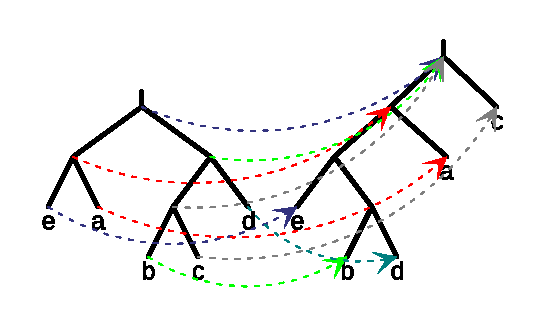
\includegraphics[width=80mm]{./pictures/mapping.pdf}
  \caption{Mapowanie $MAP_{LCA}$ dla przykładowego drzewa genów G i gatunków S.}
\end{figure}

\subsection{Drzewa DLS}

Scenariusz ewolucyjny jest przedstawieniem ewolucji danej rodziny genów, przy uwzględnieniu ewolucji gatunków, które owe geny zawierają. Jako reprezentację scenariusza ewolucyjnego można stosować drzewa nazwane drzewami DLS (\textit{Duplication-Loss-Speciation Tree}) \cite{dls}. Drzewa te posiadają dwa rodzaje węzłów wewnętrznych i dwa rodzaje liści. Pierwszy rodzaj węzła opisuje zjawisko duplikacji, czyli powielenia tego samego genu do dwóch kopii (oznaczmy jako DUP), zaś drugi jest wyrażeniem zjawiska specjacji (oznaczmy jako SPEC). Pierwszy z rodzajów liści jest opisuje stratę genu (oznaczmy jako LOSS), a drugi jest reprezentacją sekwencji genu obecnego w gatunku o danej etykiecie. Drzewo DLS dla ustalonego drzewa genów G i ustalonego drzewa gatunków S, gdzie $L(G) \subseteq L(S)$ definiuje się w następujący sposób:

\begin{enumerate}
\item \textit{s} jest drzewem DLS z jednym węzłem oznaczającym, że sekwencja genu jest obecna w gatunku \textit{s},
\item  A- jest drzewem DLS z jednym węzłem oznaczającym stratę genu, gdzie A jest niepustym zbiorem gatunków,
\item ($R_1$,$R_2$)+ jest drzewem DLS, którego korzeń jest węzłem duplikacyjnym i dzieci korzenia $R_1$ i $R_2$ są drzewami DLS takimi, że L($R_1$) = L($R_2$),
\item ($R_1$,$R_2$)$\sim$ jest drzewem DLS, którego korzeń jest węzłem specjacyjnym i dzieci korzenia $R_1$ i $R_2$ są drzewami DLS takimi, że L($R_1$) $\cap$ L($R_2$) = 0.
\end{enumerate}

Należy zaznaczyć, że z każdego drzewa DLS możliwe jest odczytanie drzewa genów za pomocą którego zostało zbudowane drzewo DLS \cite{dls}.

Klasyczną miarą kosztu ewolucyjnego danego drzewa DLS jest liczba duplikacji potrzebnych do uzgodnienia drzewa genów i gatunków.

\subsection{Scenariusz LCA}

Z wykorzystaniem mapowania LCA węzłów drzewa genów $G$ do drzewa gatunków $S$ można stworzyć drzewo DLS, które reprezentuje scenariusz LCA, to znaczy taki, który zawiera minimalną liczbę duplikacji potrzebnych do uzgodninienia drzew \cite{dowod}.

\begin{defi}
Scenariusz LCA dla drzewa $G$ o korzeniu $g$ i drzewa $S$ o korzeniu $s$, gdzie $L(G) \subseteq L(S)$, jest drzewem DLS $p(g,MAP_{LCA}(g))$, takim, że $p(g,s)$ = $s$ kiedy $g$ i $s$ są liśćmi oraz etykietą $g$ jest $s$. W innym przypadku:

\begin{equation*} 
p(g,s) =
  \begin{mcases}[ll@{\ }l]
  (p(g,u),L(T(v))-)\sim  & \text{jeśli } MAP_{LCA}(g) \in T(u), & (LOSS)\\
  (p(z,u),p(q,v))\sim    & \text{jeśli } MAP_{LCA}(z) \in T(u)\wedge MAP_{LCA}(q) \in T(v), & (SPEC)\\
  (p(z,s),p(q,s))+       & \text{jeśli } MAP_{LCA}(g) = MAP_{LCA}(z) = s, & (DUP)
\end{mcases}
\end{equation*}
gdzie \textit{u} i \textit{v} są dziećmi \textit{s} a \textit{z} i \textit{q} są dziećmi \textit{g}. 
\end{defi}

\begin{figure}[H]
  \centering
  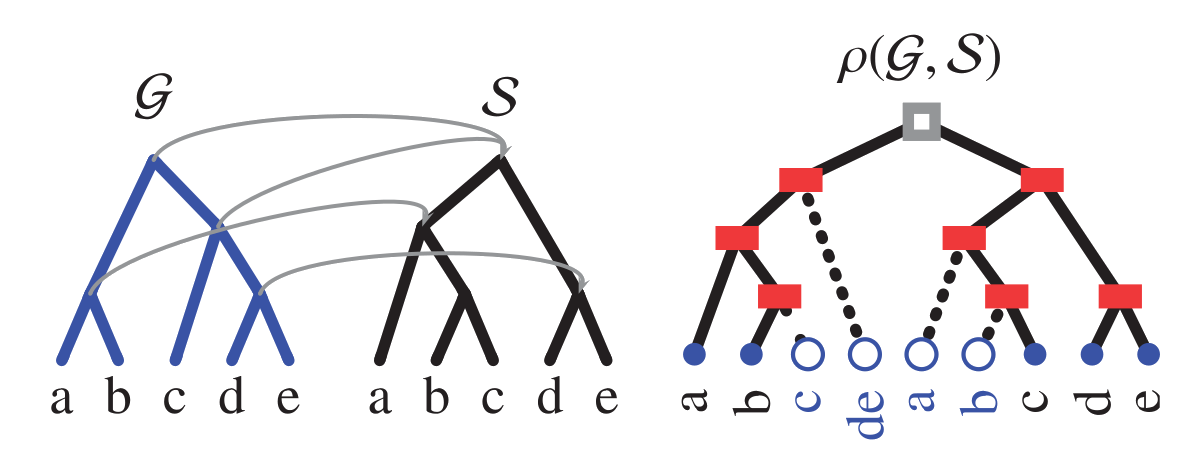
\includegraphics[width=120mm]{./pictures/DLS.png}
  \caption{Drzewo DLS $p(\mathcal{G},\mathcal{S})$ będące scenariuszem zbudowanym w oparciu o mapowanie LCA, które uzgadnia drzewo genów $\mathcal{G}$ i drzewo gatunków $\mathcal{S}$. Węzeł oznaczony szarym kwadratem jest węzłem duplikacyjnym, a czerwony kwadrat jest specjacją. Gałęzie narysowane linią przerywaną prowadzą do liści, które są reprezentacją straty genów w danym gatunku. Rysunek pochodzi z pracy \cite{dls}.}
\end{figure}

Przedstawieniem drzewa DLS jest "wbudowanie" drzewa genów, w kontener będący drzewem gatunków. 


\begin{figure}[H]
  \centering
  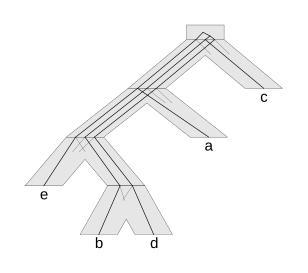
\includegraphics[width=80mm]{./pictures/optscen.png}
  \caption{Przykład wbudowania dla drzew z rysunku 1.2 \cite{gsevol}.}
\end{figure}

\section{Klastrowanie duplikacji}

Problemem podczas poszukiwania drzew DLS o najmniejszym koszcie ewolucyjnym jest odpowiednie klastrowanie duplikacji, które następują bezpośrednio po sobie. Zależnie od obranej metody klastrowania ich liczba na danym węźle drzewa gatunków może się znacząco różnić. W pracy tej zakłada się, że dzieci nie mogą znajdować się w tym samym klastrze co ojciec (klastrowanie ME). 

\begin{figure}[H]
  \centering
  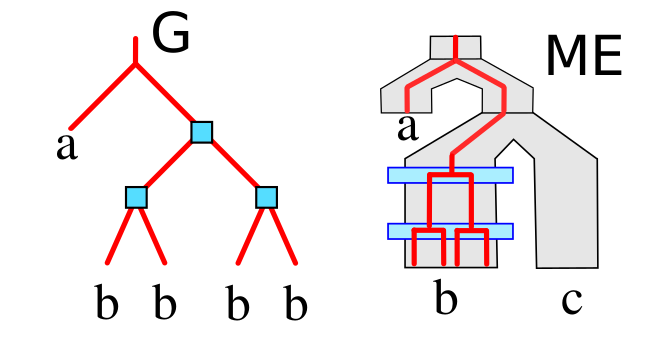
\includegraphics[width=70mm]{./pictures/clas_type_me.png}
  \caption{Klastrowanie ME dla przykładowego drzewa genów G. Rysunek zaadaptowany z pracy \cite{pasz}.}
\end{figure}



Niech S to drzewo gatunków, a $\mathcal{G}=\{G_1,G_2, ... , G_n\}$ to drzewa genów gdzie $L(G_i) \subseteq L(S)$ dla każdego $i$. Niech $\mathcal{T}=\{T_1,T_2, ... , T_n\}$ to drzewa DLS stworzone w oparciu o $\mathcal{G}$. Wówczas mówimy, że dwa węzły duplikacyjne $d_1$ i $d_2$ z $\mathcal{T}$ można sklastrować (oznaczymy jako $d_1$~$\Longleftrightarrow$~$d_2$)  jeśli poniższe warunki są spełnione:
\begin{enumerate}
\item $L(d_1) = L({d_2})$,
\item $d_1$ i $d_2$ nie leżą na jednej ścieżce (są nieporównywalne) albo $d_1=d_2$ .
\end{enumerate}

MEScore($\mathcal{T}$, S) to minimalna wielkość podziału zbioru wszystkich węzłów duplikacyjnych obecnych w scenariuszach tak, że każde dwie duplikacje z tego samego podziału są klastrowalne.

\begin{defi}\label{ME}
  MEScore($\mathcal{G}$, S) = $\min_{\cup P = Dup(\mathcal{G})} \lbrace \vert P \vert\ : \forall_{A \in P} \forall_{d_1,d_2 \in A} d_1 \Longleftrightarrow d_2 \rbrace$
 gdzie Dup($\mathcal{G}$) jest zbiorem wszystkich węzłów duplikacyjnych obecnych w $\mathcal{G}$.
 
\end{defi}
Należy wspomnieć, że klastrowanie ME nie jest jedynym możliwym rodzajem. Istnieją również klastrowania:
\begin{itemize}
\item GD, gdzie każda duplikacja musi zostać opisana jako oddzielny klaster.
\item EC, gdzie wszystkie duplikacje następujące po sobie są sklastrowane razem.
\end{itemize}
~\linebreak
Definicje na podstawie pracy \cite{pasz}.

\section{Modele scenariuszy ewolucyjnych}

Drzewo DLS, które opiera się o mapowanie LCA, jest drzewem o możliwie najmniejszym koszcie ewolucyjnym i możliwe najgłębiej położonych węzłach duplikacyjnych. Nie jest to jednak jedyny możliwy scenariusz, których w rzeczywistości jest nieskończenie wiele. Należy jednak pamiętać, że nie powinno się brać pod uwagę przypadków skrajnie nieprawdopodobnych, gdzie gen jest, dla przykładu, wielokrotnie duplikowany i tracony. Po wprowadzeniu tego typu ograniczeń możliwe jest otrzymanie skończonego zbioru możliwych scenariuszy ewolucyjnych, które zwane są semi-normalnymi. Formalnie drzewo DLS nazywamy semi-normalnym jeśli:
\begin{enumerate}
\item nie istnieje węzeł duplikacyjny, którego dzieckiem jest strata,
\item nie istnieje węzeł specjacyjny, którego dzieci są stratami.
\end{enumerate}


\subsection{Transformacje scenariuszy ewolucyjnych}

Drzewo DLS podlega ściśle określonym transformacjom (zwanych również ruchami), które zmieniają jego strukturę, ale zachowując poprawność danego drzewa: 
\begin{enumerate}
\item TMOVE: $((C-,P)\sim,(C-,Q)\sim))+   \Longrightarrow    (C-,(P,Q)+)\sim $ ,
\item CLOST: $((P,Q-)\sim,(P-,Q)\sim)+   \Longrightarrow   (P,Q)\sim $ ,
\end{enumerate}
gdzie $C,P,Q$ są drzewami DLS.

\begin{figure}[H]
  \centering
  \includegraphics[width=120mm]{./pictures/move.png}
  \caption{Ruchy TMOVE i CLOST wraz z ich biologiczną interpretacją. Szary  kwadrat reprezentuje duplikację. Czerwony prostokąt i czerwona linia przerywana są reprezentacją specjacji, a niebieskie koło jest stratą. Rysunek zaadaptowany z pracy \cite{dls}.}
\end{figure}



Stosowane są również odwrotności zdefiniowanych powyżej transformacji, które oznaczone są indeksem górnym~$^{-1}$ np. TMOVE$^{-1}$.

Dla ustalonego drzewa genów G i ustalonego drzewa gatunków S, gdzie $L(G) \subseteq L(S)$, możliwe jest uzyskanie zbioru scenariuszy semi-normalnych, który reprezentowany jest jako zbiór drzew DLS, poprzez zastosowanie ruchów TMOVE$^{-1}$ i CLOST$^{-1}$ na drzewie DLS będącym scenariuszem LCA. 

Na rysunku 1.7 przedstawione są wszystkie możliwe przekształcenia TMOVE i CLOST dla przykładowych drzew G i S.

\subsection{Opis modeli dopuszczalnych scenariuszy}

W praktyce nie zawsze rozważa się wszystkie możliwe scenariusze do klastrowania, ponieważ może prowadzić to do nieprawdopodobnych klastrowań duplikacji np. gdzie wszystkie duplikacje ulokowane zostały w korzeniu drzewa DLS. 

W literaturze wyodrębniono kilka dopuszczalnych modeli, a w pracy tej zajęto się podanymi niżej modelami, które dopuszczają podane warunki:
\begin{enumerate}
\item Model PG \cite{pasz}: Model ten dopuszcza tylko takie drzewa DLS, które zachowują minimalny koszt duplikacyjny. Oznacza to, że są to scenariusze osiągalne ze scenariusza LCA reprezentowanego drzewem DLS za pomocą transformacji TMOVE$^{-1}$.
\item Model FHS \cite{pasz}: Model ten dopuszcza każde możliwe przekształcenie drzew DLS, nawet jeśli takie drzewo nie zachowuje minimalnego kosztu duplikacyjnego. Oznacza to, że są to scenariusze osiągalne ze scenariusza LCA reprezentowanego drzewem DLS za pomocą transformacji TMOVE$^{-1}$ i CLOST$^{-1}$.
\end{enumerate}

\begin{figure}[H]\label{diagram_red}
  \centering
  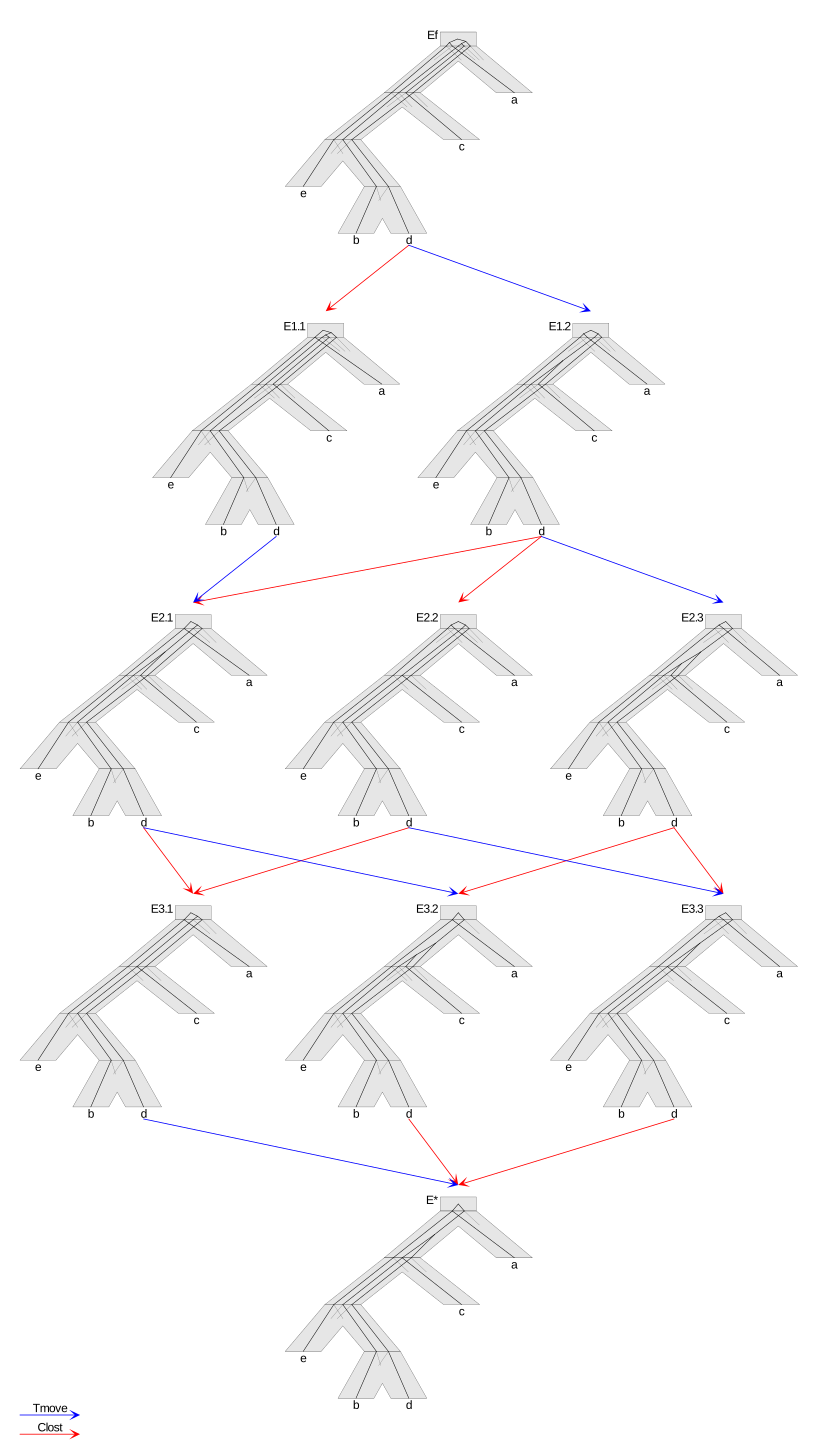
\includegraphics[width=\textwidth,height=\textheight,keepaspectratio]{./pictures/diagram_1.png}
  \caption{Diagram przekształceń scenariuszy semi-normalnych. Na dole rysunku, oznaczone filetowym kołem, znajduje się drzewo uzyskane za pomocą mapowania LCA. Model PG zawierać będzie tylko drzewa oznaczone zielonym kołem, podczas gdy dla modelu FHS wszystkie drzewa obecne na diagramie są częścią zboru scenariuszy semi-normalnych \cite{gsevol}.}
\end{figure}

\chapter{Heurystyka}\label{r:heurystyka}

\section{Opis problemu}

\section{Opis algorytmu}

\begin{algorithm}[H]
 \KwIn{
 \begin{enumerate}
\item Drzewo gatunków $S$ z~węzłami $<s_1,s_2, ... , s_m>$,
\item Drzewa genów $G_1,G_2, ... , G_z$ gdzie $L(G_i) \subseteq L(S)$,
\item Dla każdego drzewa genów $G_i$ zbiór scenariuszy $R_i$ w~postaci wektorów $<{e_i}^1,{e_i}^2, ... , {e_i}^m>$, gdzie dla każdego $j$, ${e_i}^j$ to liczba epizodów duplikacyjnych przypisanych do węzła $s_j$ w~$i$-tym scenariuszu.
\end{enumerate}}
 \KwOut{\begin{enumerate}
 \item Scenariusz w postaci wektora $<{e}^1,{e}^2, ... , {e}^m>$, gdzie dla każdego $j$, ${e}^j$ to minimalna liczba epizodów duplikacyjnych przypisanych do węzła $s_j$.
 \end{enumerate}}
 $V^{max}$ = wektor $<{e}^1,{e}^2, ... , {e}^m>$, gdzie dla każdego $j$, ${e}^j$ to maksymalna liczba epizodów duplikacyjnych przypisanych do węzła $s_j$ w każdym scenariuszu $R_i$ dla każdego drzewa $G$.\;
 $V^*$ = $V^{max}$\;
 \For{$s_x \in S$ w ustalonej kolejności}{
  ${V_{new}}^*$ = $V^*$\;
  \While{zmiana w węźle ${V_{new}}^*[s_x]$ i ${V_{new}}^*[s_x] > 0$}{
  ${V_{new}}^*$[$s_x$] - -\;
  \If{${V_{new}}^* \subseteq R_i$ dla każdego drzewa $G$}{
   $V^*$ = ${V_{new}}^*$\;
   }
   }
 }

\end{algorithm}

Wybór współrzędnej może, zależnie od potrzeby, może być dokonywany w inny sposób:
\begin{itemize}
\item od końca wektora (od korzenia),
\item od początku (od liści),
\item losowo.
\end{itemize}

\section{Dokumentacja użytkowa i~opis implementacji}\label{r:impl}
Opisana heurystyka zaimplementowana została w języku Python w wersji 3.7.4 przy użyciu paradygmatu obiektowego, gdzie zbiór wszystkich drzew DLS dla wszystkich drzew, zbiór drzew semi-normalnych otrzymanych z jednego drzewa genów, a także pojedyncze drzewo DLS stanowią oddzielne klasy. Fragment kodu można zobaczyć w dodatku A. Program pythonowy przyjmuje na wejściu listę plików w których zawarte są wyliczone scenariusze dla danego drzewa genów.

Algorytm ten, dla wygody użycia, został obudowany skryptem napisanym w języku bash, który pozwala na wyliczenie scenariuszy w modelu FHS i PG z wykorzystaniem programu DLSgen autorstwa dra hab. Pawła Góreckiego.\cite{dlsgen} Program ten wylicza dla danego drzewa genów i drzewa gatunków scenariusze ewolucyjne, które wykorzystywane są jako dane wejściowe dla proponowanej heurystyki.


\section{Testy algorytmu}
Do sprawdzenia wyników wyliczanych przez proponowany algorytm użyty został program RME napisany przez dra Jarosława Paszka. Program ten korzystając z dostępnych metod algorytmicznych wylicza dokładne i najniższe możliwe wartości kosztu ewolucyjnego dla podanych modeli z użyciem klastrowania ME. \cite{rme}
\\
Z powodu trudności w obliczeniu danych wejściowych dla heurystyki obecnie nie ma możliwości dla przetestowania algorytmów dla dużych zbiorów danych.
\\
Ze względu na czytelność wykresów w dalszej części pracy we wszystkich testach uwzględniony został tylko losowy wybór współrzędnej. W trakcie testów okazało się również, że taki wybór prowadzi zawsze do najlepszych wyników. 


\subsection{Testy algorytmu na danych rzeczywistych}
Zbiorem danych dla testu na danych rzeczywistych był zbiór Guigo zawierający 53 ukorzenione drzewa genów pochodzące od 16 eukariontów. Do zbioru tego załączono dwa drzewa gatunków $S_1$ z pracy \cite{guigo} i $S_2$ z pracy \cite{guigo_2}. 

\begin{figure}[H]
\centering
\begin{subfigure}{.5\textwidth}
  \centering
  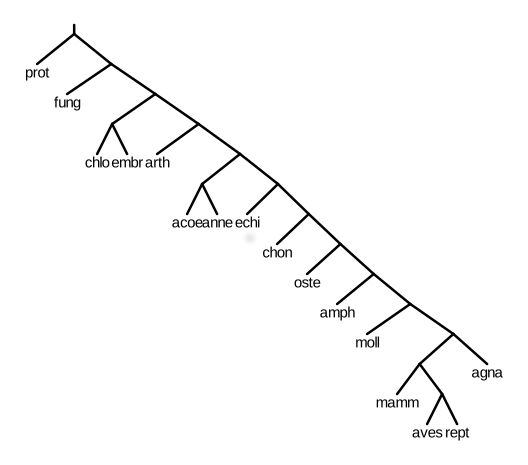
\includegraphics[width=50mm]{./pictures/guigo_spec_1.png}
  \caption{Drzewo $S_1$}
\end{subfigure}%
\begin{subfigure}{.5\textwidth}
  \centering
  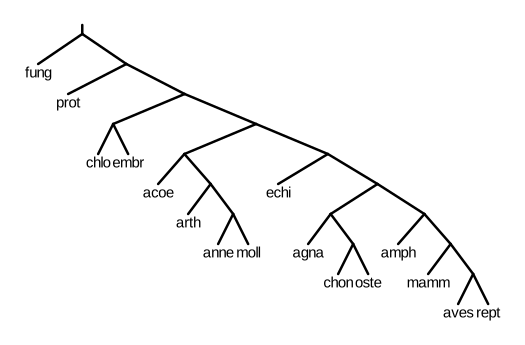
\includegraphics[width=50mm]{./pictures/guigo_spec_2.png}
  \caption{Drzewo $S_2$}
\end{subfigure}%
\caption{Drzewa gatunków ze zbioru Guigo}
\end{figure}

\begin{figure}[H]
\centering
\begin{subfigure}{.5\textwidth}
  \centering
  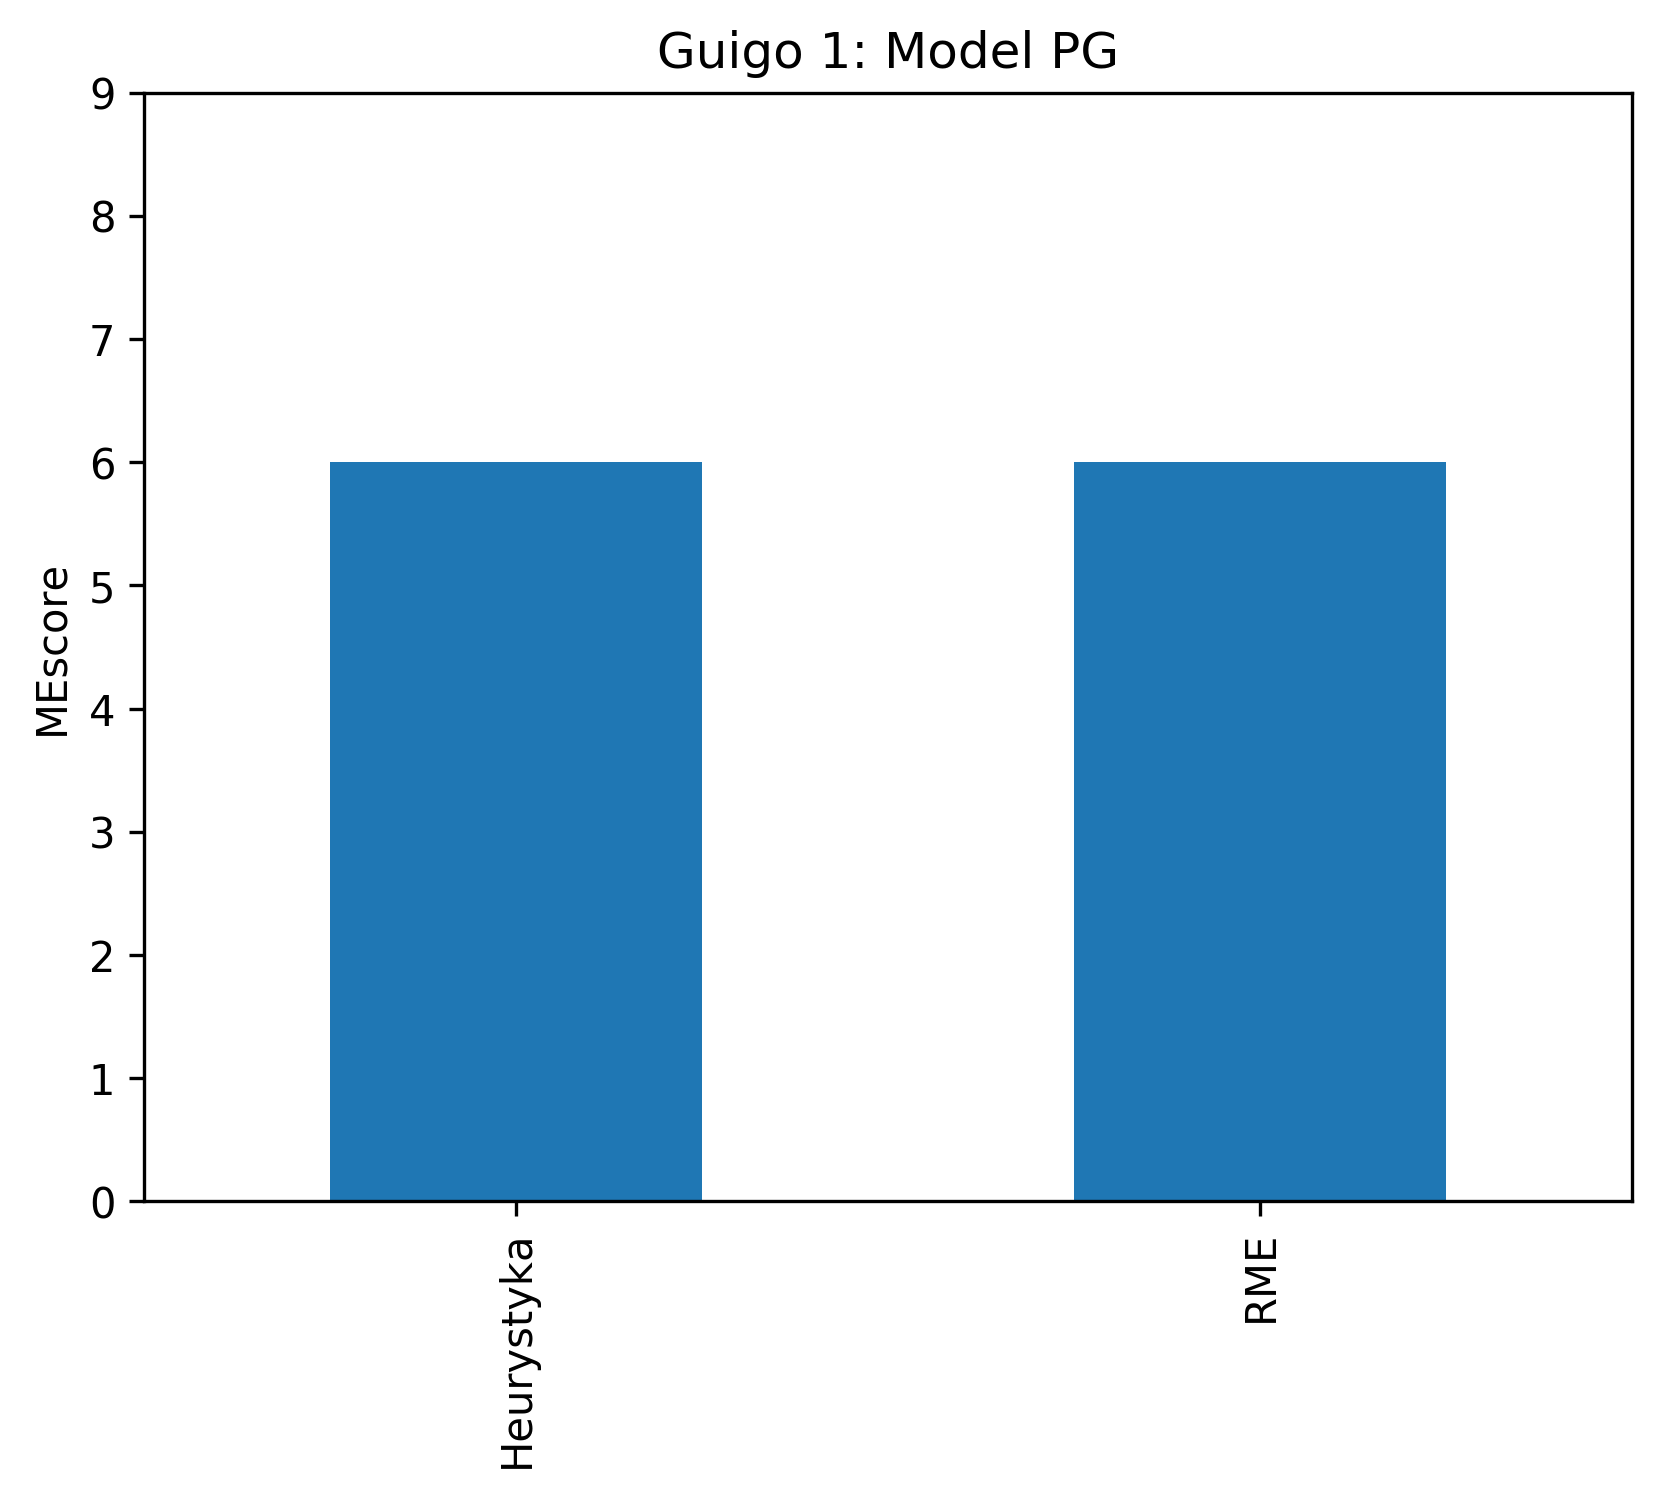
\includegraphics[width=50mm]{./pictures/G1_PG.png}
  \caption{Test algorytmu dla modelu PG}
\end{subfigure}%
\begin{subfigure}{.5\textwidth}
  \centering
  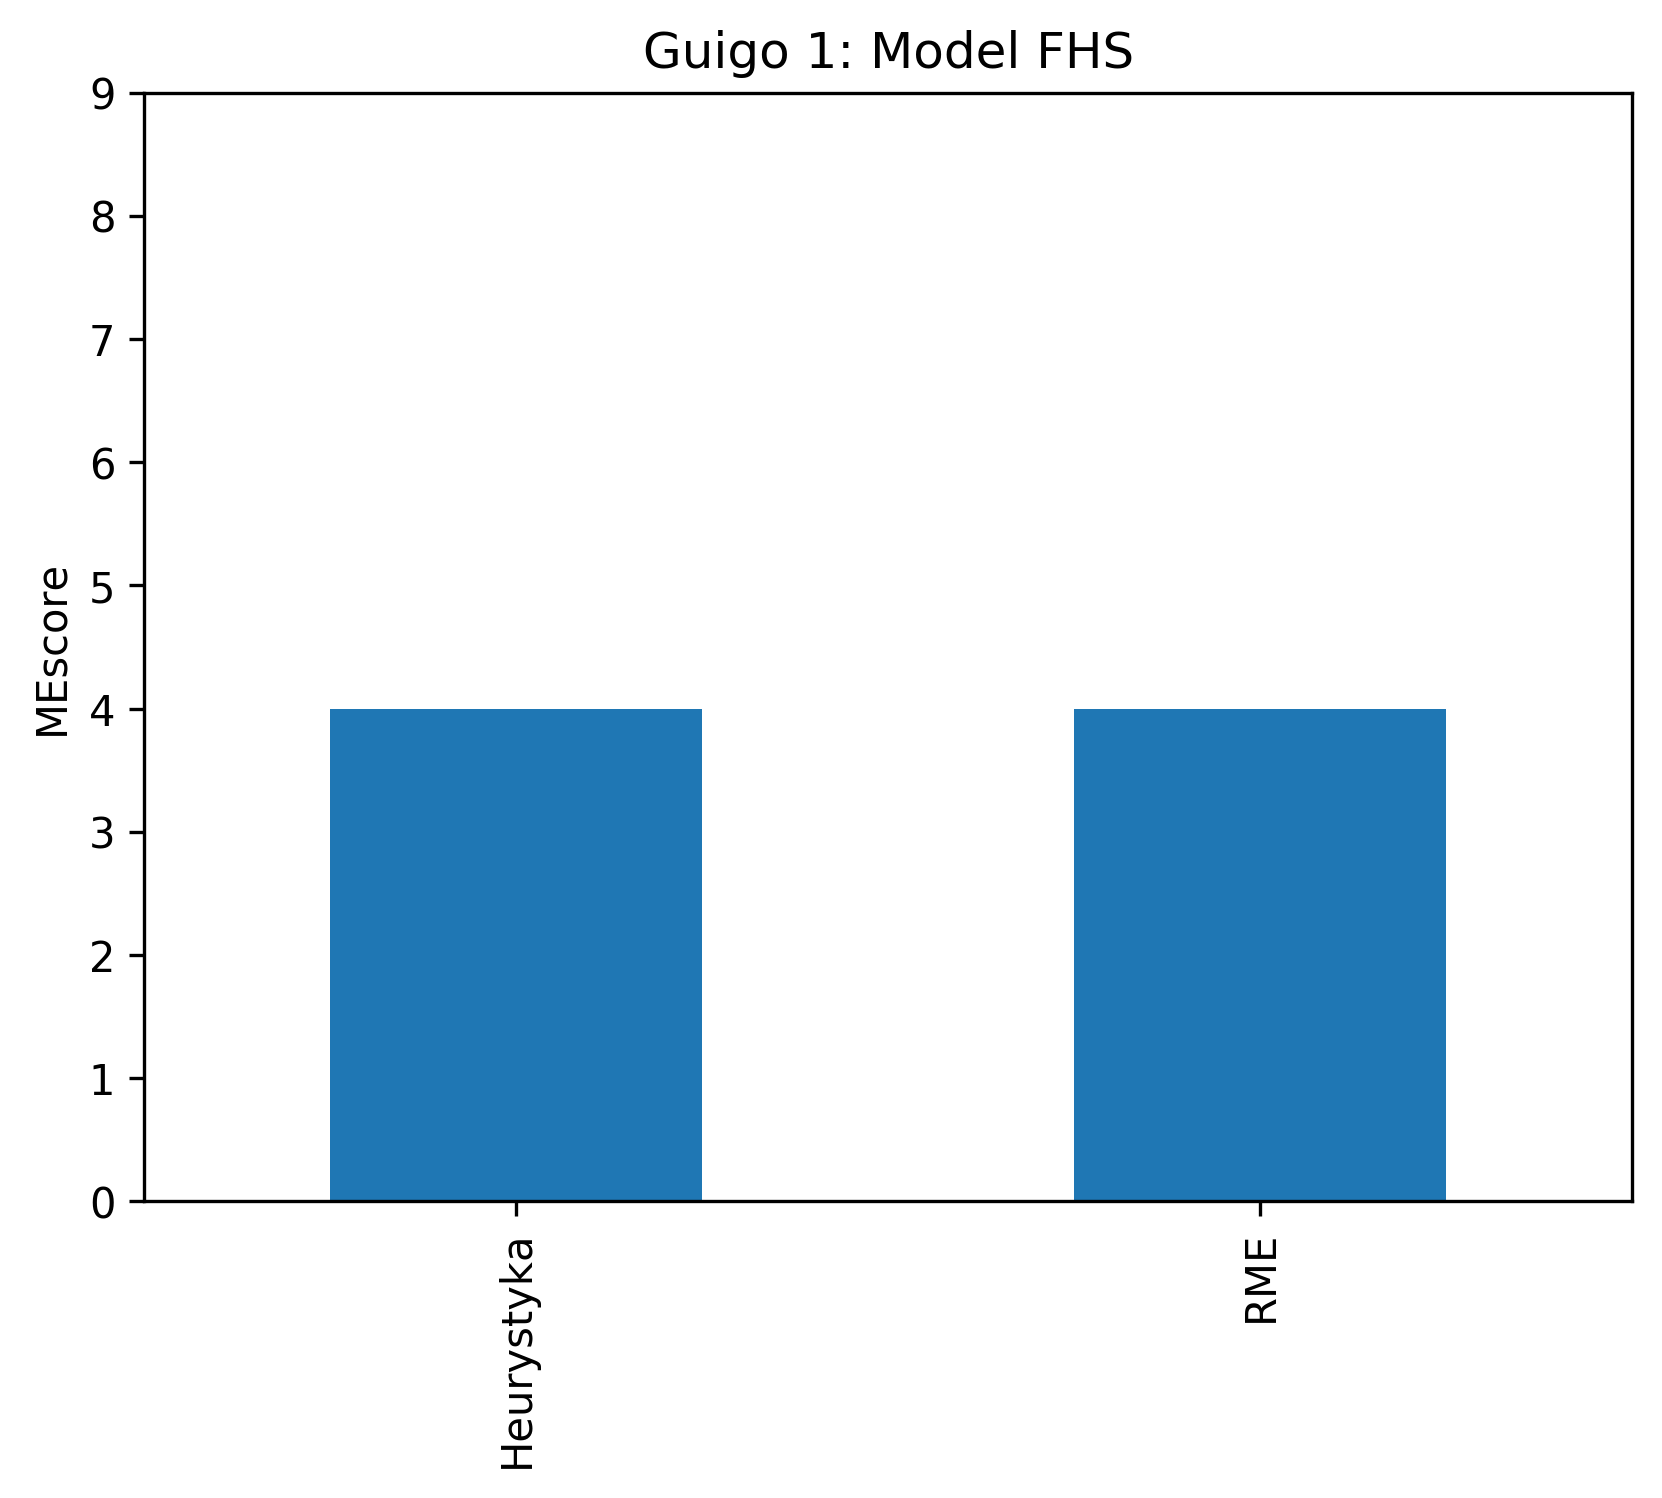
\includegraphics[width=50mm]{./pictures/G1_FHS.png}
  \caption{Test algorytmu dla modelu FHS}
\end{subfigure}%
\caption{Testy algorytmu na danych rzeczywistych dla drzewa gatunków $S_1$}
\end{figure}


\begin{figure}[H]
\centering
\begin{subfigure}{.5\textwidth}
  \centering
  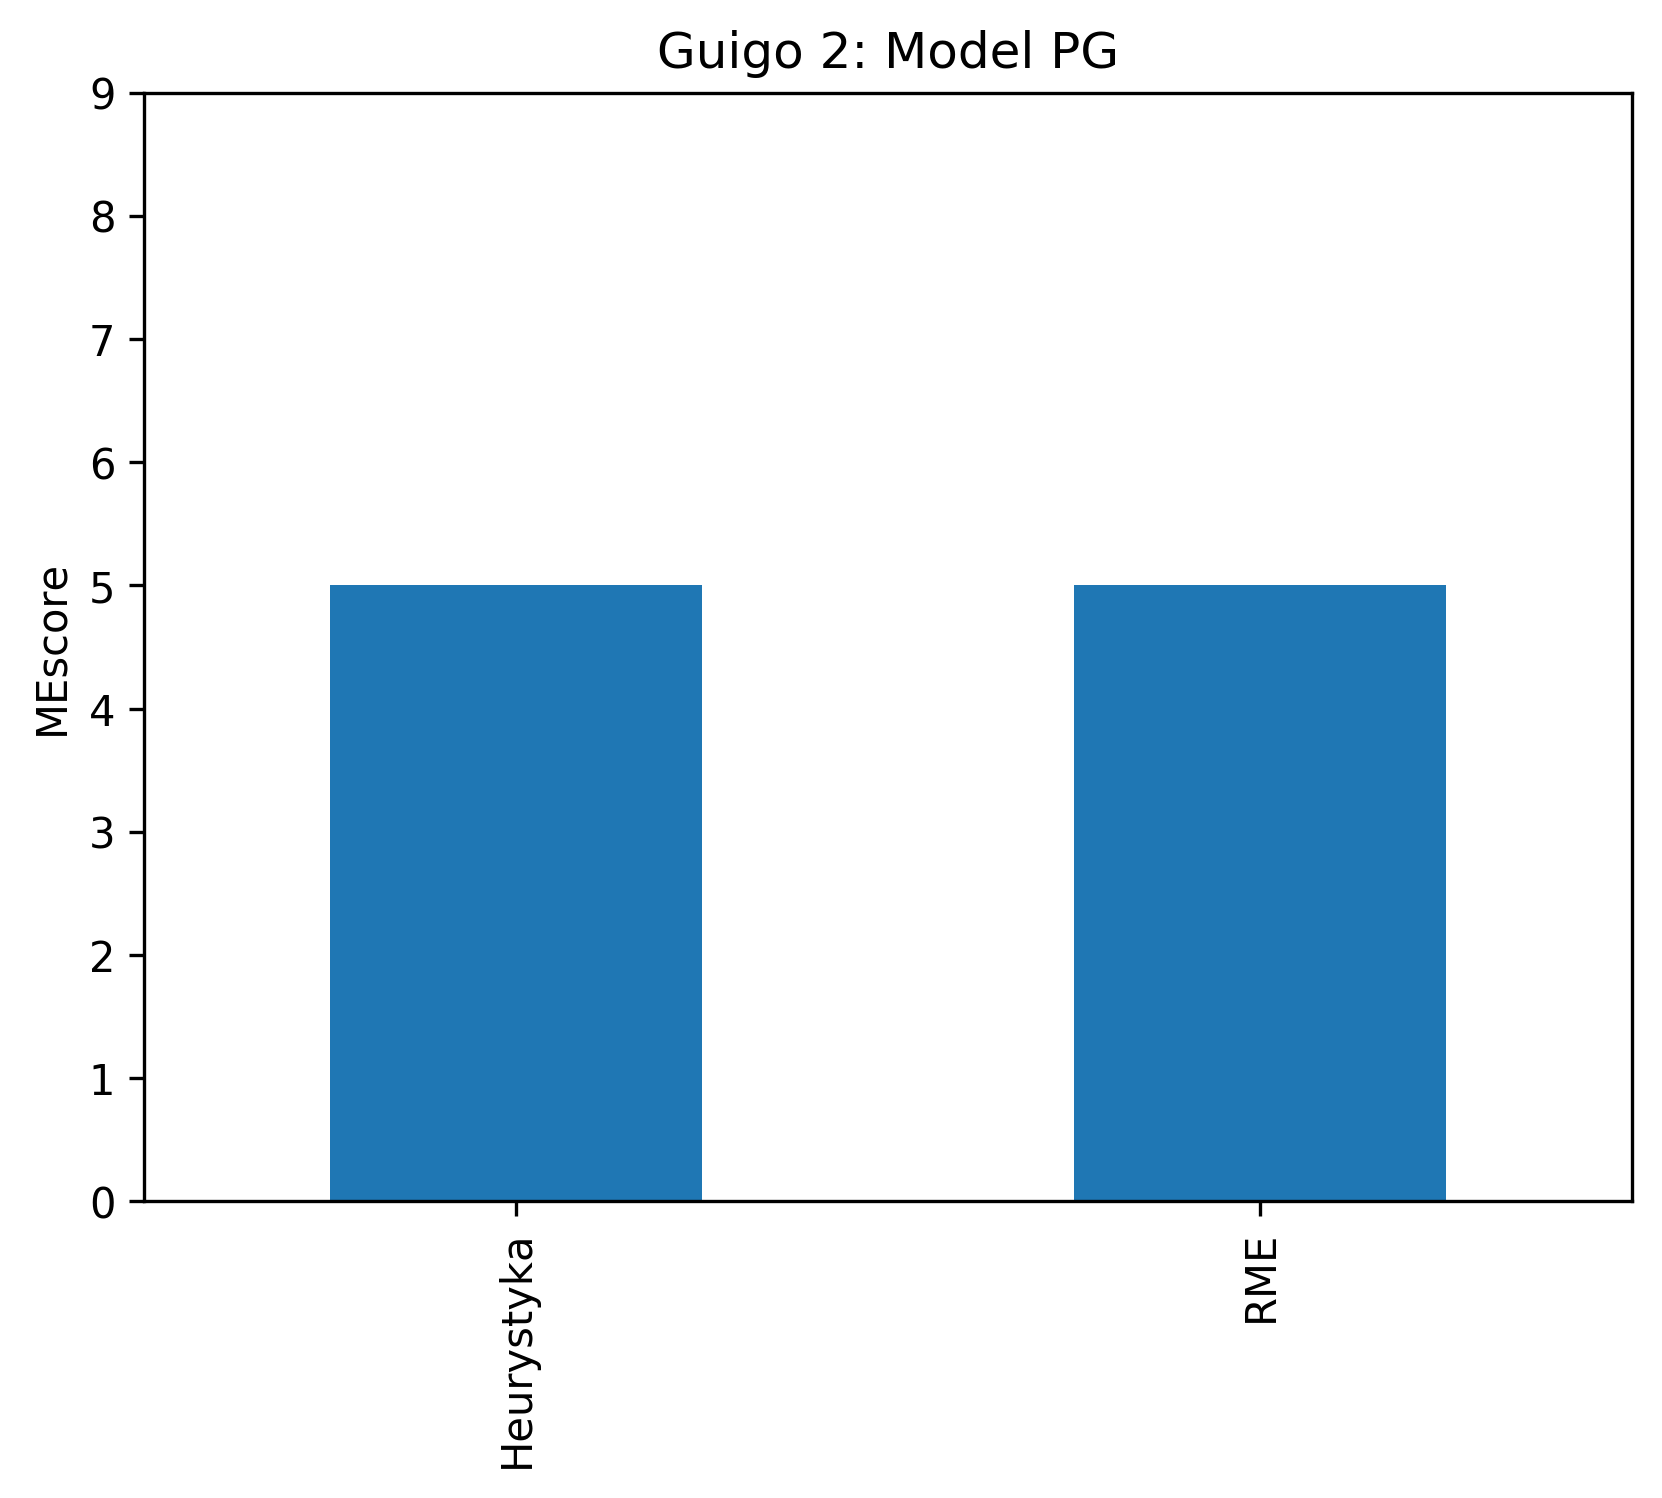
\includegraphics[width=50mm]{./pictures/G2_PG.png}
  \caption{Test algorytmu dla modelu PG}
\end{subfigure}%
\begin{subfigure}{.5\textwidth}
  \centering
  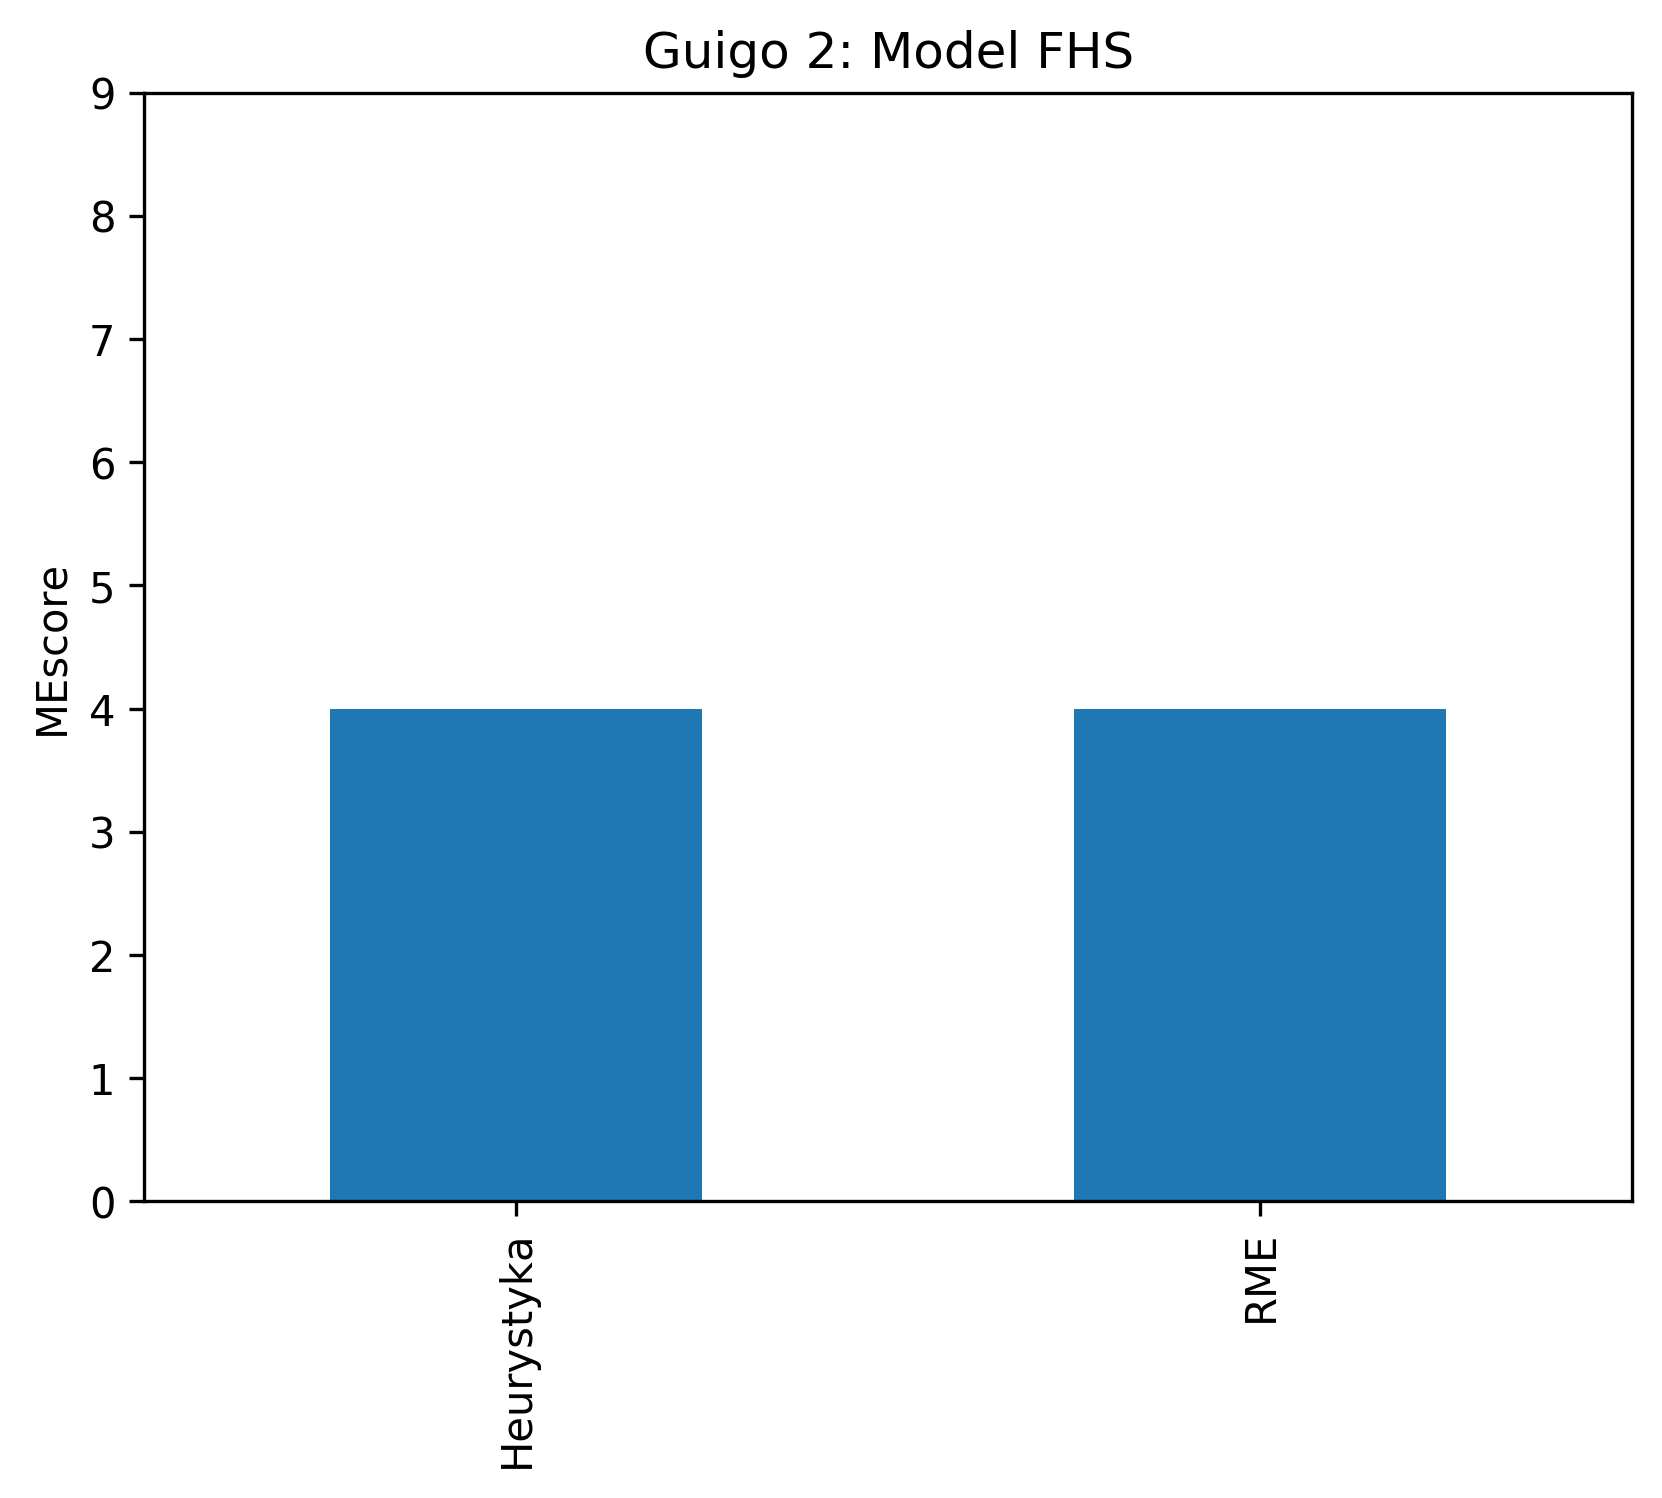
\includegraphics[width=50mm]{./pictures/G2_FHS.png}
  \caption{Test algorytmu dla modelu FHS}
\end{subfigure}%
\caption{Testy algorytmu na danych rzeczywistych dla drzewa gatunków $S_2$}
\end{figure}

Dla wszystkich przypadków algorytm przy losowym wyborze współrzędnych jest w stanie osiągnąć wyniki identyczne jak te wyliczone przez program RME. 

\subsection{Testy algorytmu na danych symulowanych}
Dane dla testów syntetycznych zostały wygenerowany w sposób losowy jednak wielkość, struktura i ilość drzew genów zostały dopasowane do zbioru Guigo. Zbiory symulowane zawierają syntetyczne drzewo gatunków z 15 liśćmi oraz  wygenerowane losowo, w oparciu o algorytm YULA, 48 ukorzenione drzewa genów etykietowane gatunkami z wylosowanego wcześniej drzewa gatunków. Przykładowe drzewa gatunków (w formie graficznej) i genów (w formie tekstowej) można znaleźć w dodatkach do pracy. Test został przeprowadzony dla 1000 losowych zestawów.

\begin{figure}[H]
\centering
\begin{subfigure}{.5\textwidth}
  \centering
  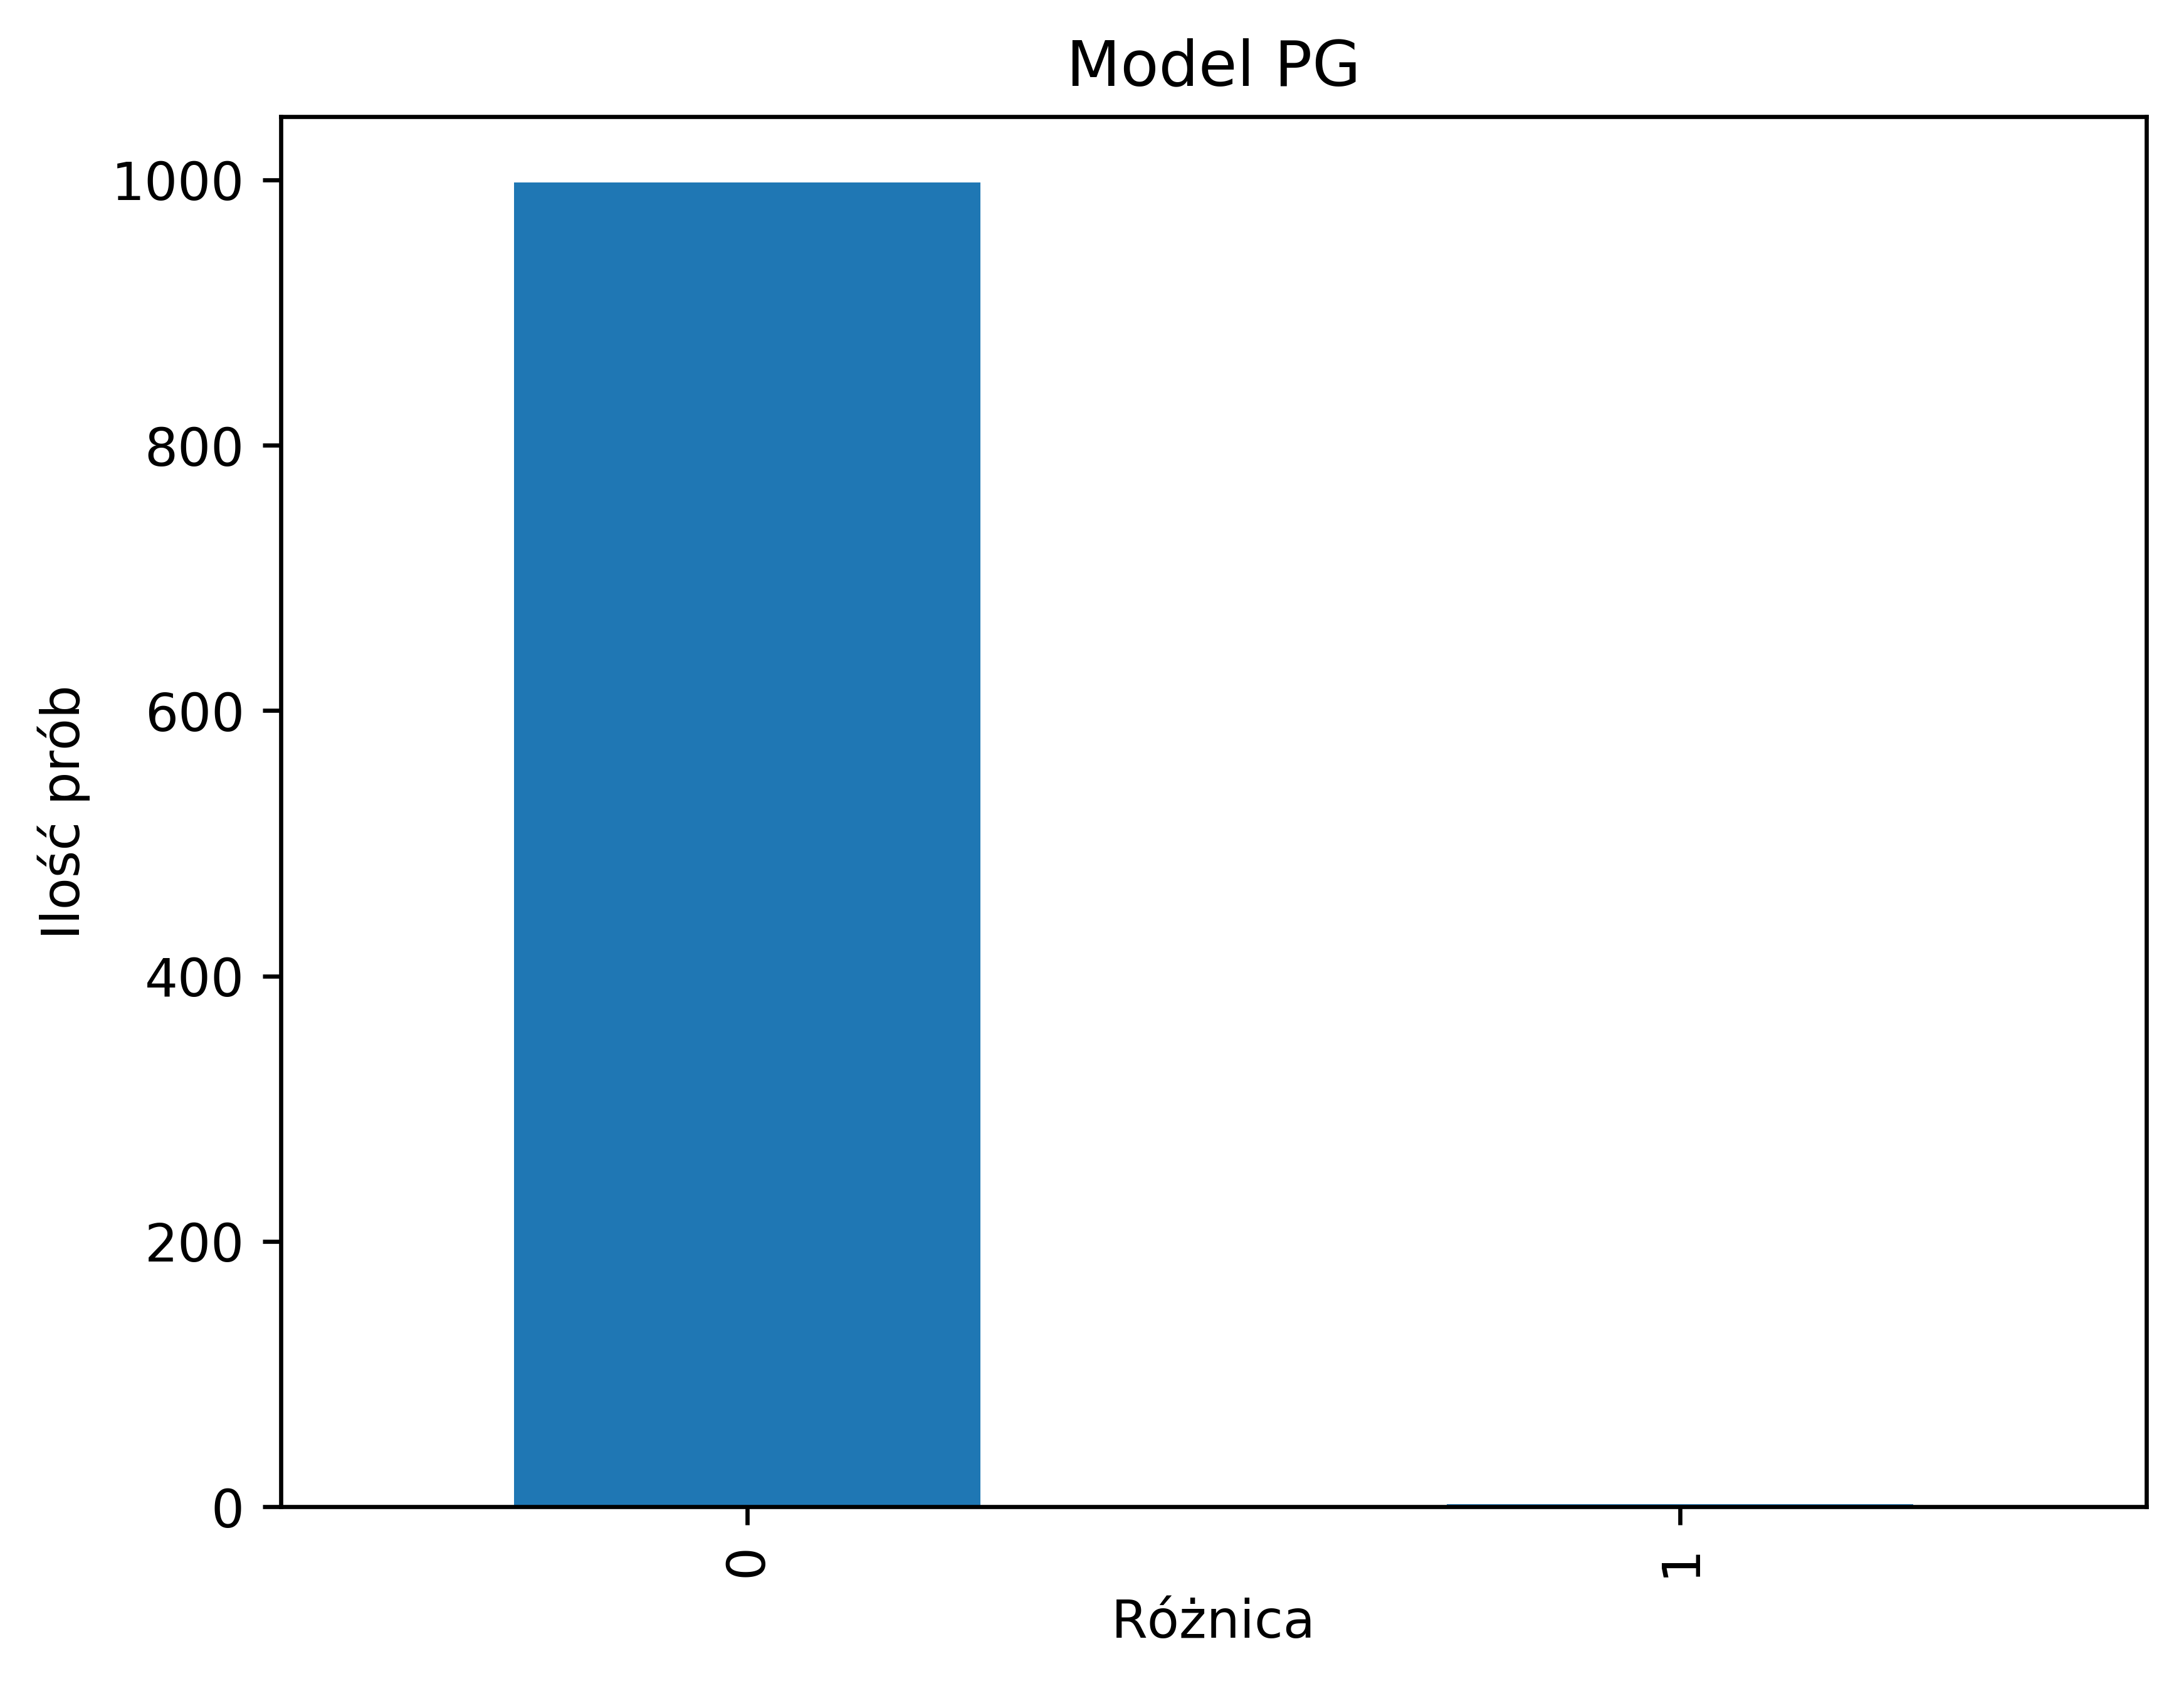
\includegraphics[width=50mm]{./pictures/PG.png}
  \caption{Test algorytmu dla modelu PG}
\end{subfigure}%
\begin{subfigure}{.5\textwidth}
  \centering
  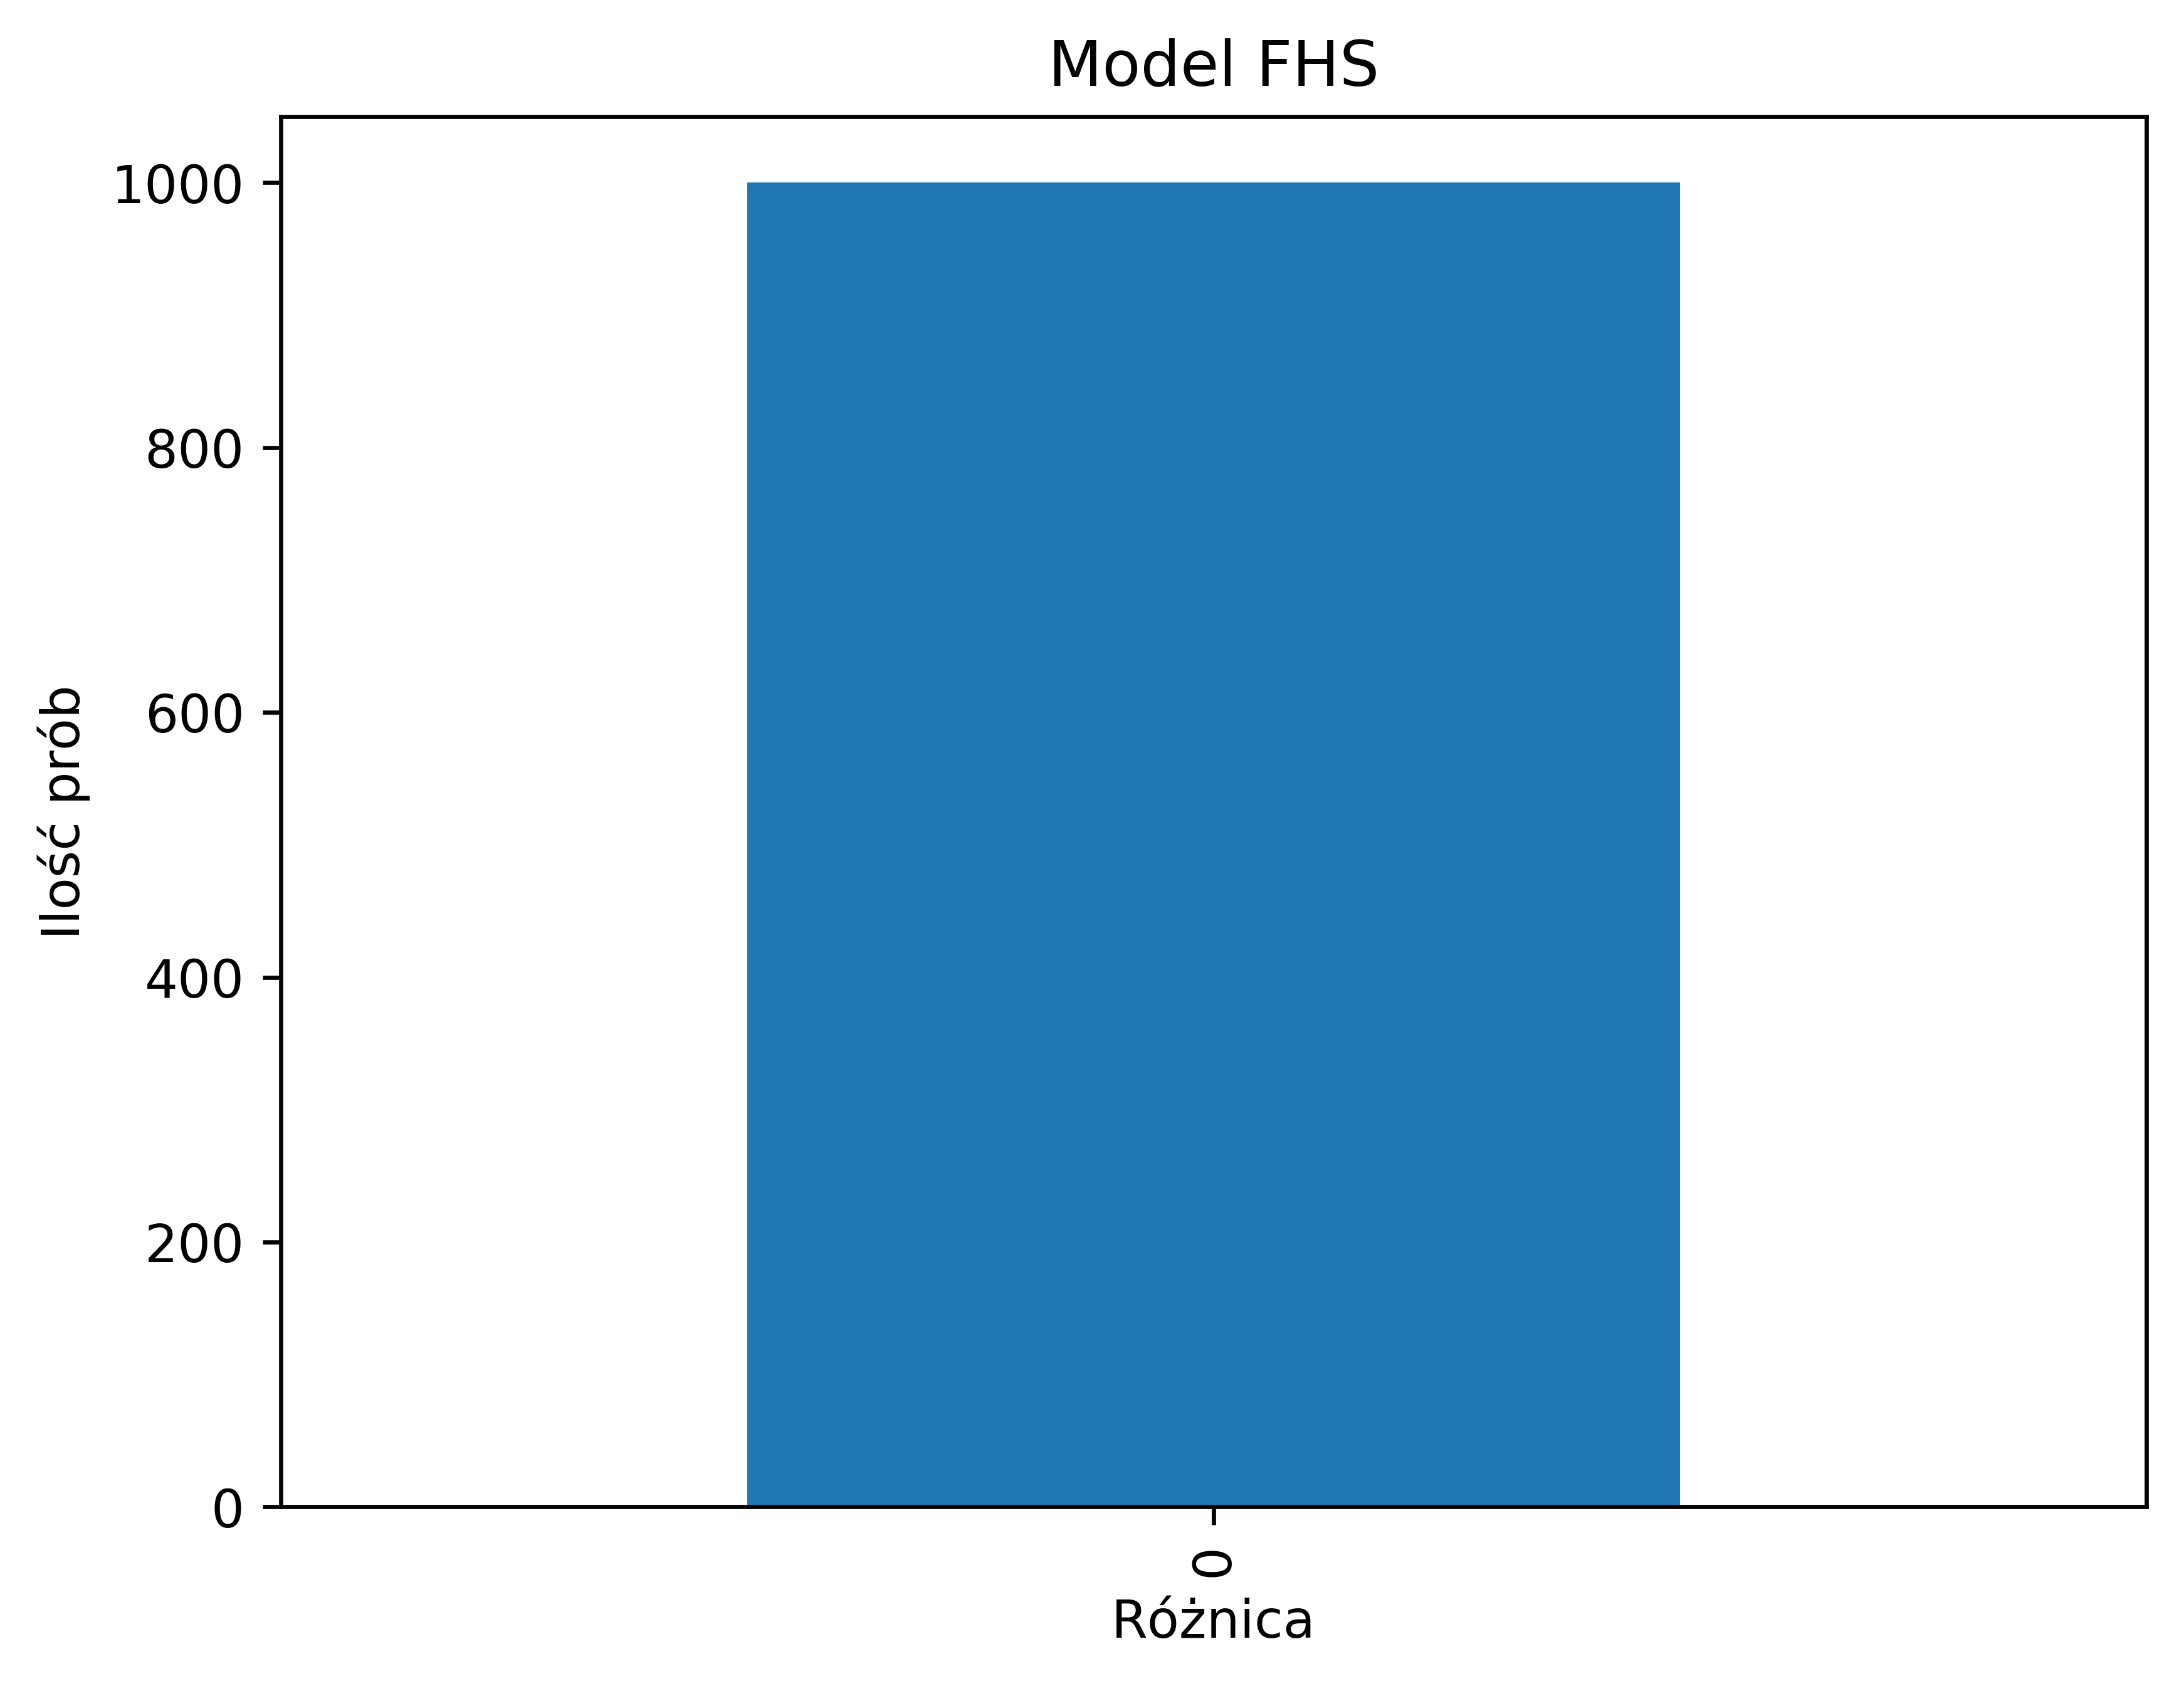
\includegraphics[width=50mm]{./pictures/FHS.png}
  \caption{Test algorytmu dla modelu FHS}
\end{subfigure}%
\caption{Testy algorytmu na danych symulowanych. Przez różnicę rozumiany jest wynik odjęcia od wyliczeń otrzymanych przez program RME wyliczeń otrzymanych dzięki proponowanemu algorytmowi. }
\end{figure}

W obu przypadkach wyniki obliczeń heurystyki nie odbiegają znacząco od dokładnych wartości kosztu ewolucyjnego otrzymanych przez program RME. Za pomocą wykresu nie da się nawet dokładnie określić dla ilu zbiorów heurystyka nie wyliczyła prawdziwego, minimalnego kosztu.\\
Dla modelu PG tylko 4 zbiory z 1000 nie dały tego samego wyniku, a dla modelu FHS było to 17 zbiorów z 1000.

\chapter{Podsumowanie}

W~pracy przedstawiono pierwszy i dosyć intuicyjny pomysł na ocenę scenariuszy ewolucyjnych reprezentowanymi drzewami DLS pod kątem ilości duplikacji. Należy jednak wspomnieć, że samą ideę da się znacząco usprawnić i obniżyć złożoność obliczeniową być może nawet do poziomu liniowego. 
\\.  W związku z tym trudno mówić o czasie potrzebnym algorytmowi na własne obliczenia. Nie udało się zaobserwować, by algorytm kiedykolwiek potrzebował
Obecnie to właśnie krok w którym konieczne jest wyliczenie scenariuszy dla drzew genów jest krokiem najbardziej wymagającym czasowo i obliczeniowo.  W związku z tym trudno mówić o czasie potrzebnym algorytmowi na własne obliczenia. Nie udało się zaobserwować, by algorytm kiedykolwiek potrzebował więcej niż jedną sekundę na wczytanie danych i więcej niż 0.3 sekundy na obliczenie drzewa o najmniejszym koszcie ewolucyjnym. Ponadto obecne wymaganie dotyczące danych wejściowych uniemożliwia  przetestowanie algorytmu na danych bardziej złożonych niż zbiór Guigo. 
\\
Testy pokazują również, że opisany algorytm zwraca wyniki, które różnią się w bardzo niewielkim stopniu od rzeczywistego minimalnego kosztu ewolucyjnego, gdyż maksymalnie tylko dla 2,8\% danych algorytm nie uzyskał najniższego możliwego wyniku. Maksymalna różnica jaką udało się zaobserwować wynosiła 1, co również nie jest dużą wartością. Może to jednak wynikać z dosyć niskiego kosztu ewolucyjnego drzew DLS zawartych w badanych zbiorach, który wynosił maksymalnie 9 (średnia arytmetyczna = 6,1) dla modelu PG i 7 (średnia arytmetyczna = 4,5) dla modelu FHS. Obserwowalne jest, że proponowany algorytm wymaga kolejnych, bardziej rozbudowanych testów.


\section{Perspektywy rozwoju}

Trudno przewidzieć wszystkie możliwości rozwoju algorytmu, ale te bardziej
oczywiste można wskazać już teraz.  Są to:
\begin{itemize}
\item Uniezależnienie algorytmu od kroku w którym wyliczane są scenariusze i klastrowanie duplikacji bezpośrednio na podstawie drzew genów.
\item Uliniowienie algorytmu.
\end{itemize}

Szczególnie punkt pierwszy proponowanych usprawnień jest kluczowy dla dalszego rozwoju heurystyki, ponieważ pozwoli on na używanie i przeprowadzenie testów dla danych dużo bardziej skomplikowanych i bardziej przystających do obecnych problemów niż zbiór Guigo.

\section{Perspektywy wykorzystania}

Podstawową zaletą przedstawionej heurystyki jest jej elastyczność. Ocena scenariuszy nie zależy od obranego modelu, a obecnie wydaje się, że same obliczenia nie są obarczone dużym błędem. Kolejną niewątpliwą zaletą jest fakt, że w istocie również struktura drzewa nie ma dla algorytmu dużego znaczenia. Obecnie powoli odchodzi się od drzewa binarnego jako metody przedstawienia historii ewolucji i algorytm jest na taką zmianę gotowy. Z punktu widzenia algorytmu drzewa są tablicą zawierającą ilość klastrów duplikacyjnych dla danego węzła, a które umieszczone są w niej w porządku prefiksowym, co zapewnia możliwość wykorzystania algorytmu nie tylko dla drzew binarnych. Algorytm funkcjonuje obecnie jednak w dosyć prymitywnej formie i wymaga wzmożonej i dokładnej pracy, ale sam algorytm rokuje niezwykle pozytywnie.  

\appendix

\chapter{Pętla programu zapisana w~języku Python wykonywana dla losowego wybierania indeksów}

\begin{verbatim}

		max_trees = []
        for scenario in self:
            all_dup_pref = [tree.duplication_prefix for tree n scenario]
            max_trees.append(self.rate_scenario(all_dup_pref))
        max_tree = self.rate_scenario(max_trees)

        if select_type == "random":

            index_list = [x for x in range(len(max_tree)) if x != 0]

            while index_list:
                index_list_position = random.randint(0, len(index_list) - 1)
                index = index_list[index_list_position]

                max_tree_temp = max_tree[:]
                max_tree_temp[index] -= 1

                for scenario in self:
                    for tree in scenario:
                        for i in range(len(tree.duplication_prefix)):
                            if max_tree_temp[i] - tree.duplication_prefix[i] < 0:
                                break
                        else:
                            break
                    else:
                        index_list.pop(index_list_position)
                        break
                else:
                    max_tree = max_tree_temp
            return max_tree, sum(max_tree)
\end{verbatim}

\chapter{Przykładowe drzewa gatunków dla danych syntetycznych}



\begin{figure}[H]
  \centering
  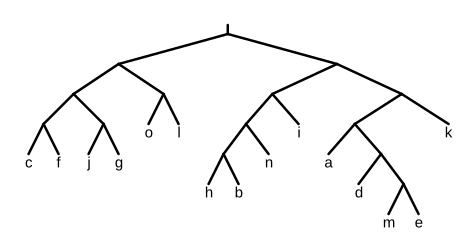
\includegraphics[width=80mm]{./pictures/syn_spec_1.png}
  \caption{Drzewo gatunków $S_1$}
\end{figure}

\begin{figure}[H]
  \centering
  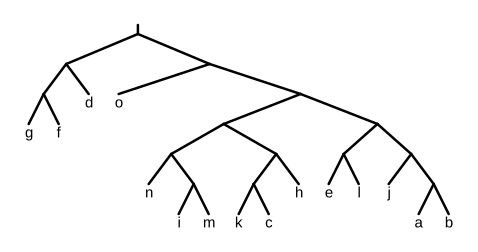
\includegraphics[width=80mm]{./pictures/syn_spec_2.png}
  \caption{Drzewo gatunków $S_2$}
\end{figure}


\chapter{Przykładowe drzewa genów dla danych syntetycznych}
\begin{obeylines}
Format tekstowy:
((b,l),h)
((a,k),b)
((i,k),a)
((l,b),o)
(h,(j,o))
(b,(i,c))
(b,(m,j))
((m,a),b)
((g,m),f)
((a,l),k)
(o,(j,h))
((k,d),i)
(e,(c,o))
(f,(a,h))
(j,(k,d))
((k,e),c)
(j,(e,b))
((i,n),l)
(f,(b,h))
(c,(k,g))
((l,o),j)
((a,f),d)
((f,h),j)
(h,(d,n))
((b,j),i)
((a,e),(g,l))
((b,c),(n,o))
(m,((j,h),d))
((e,(f,g)),a)
(((m,d),g),a)
((h,l),(n,b))
((d,(b,a)),k)
(((k,n),c),m)
(((d,c),b),(j,a))
(c,((l,(g,j)),k))
(((h,g),(a,e)),l)
((o,(f,e)),(j,h))
((g,l),((c,m),n))
((e,(f,(j,o))),k)
(f,(a,((n,h),(b,c))))
((a,(o,h)),((e,i),n))
((e,d),((a,b),(n,g)))
(((m,(d,b)),j),(f,e))
((l,h),(((a,j),((m,g),f)),e))
((n,(i,e)),(((a,k),f),(l,b)))
((j,e),(i,((a,(k,(l,d))),n)))
((((f,k),(b,(o,e))),((g,n),j)),m)
(h,((b,(m,f)),((c,j),(a,(k,l)))))
\end{obeylines}

\begin{thebibliography}{99}
\addcontentsline{toc}{chapter}{Bibliografia}

\bibitem[1]{gsevol} Wygenerowane za pomocą serwisu: http://gsevol.azor.mimuw.edu.pl 

\bibitem[2]{rme} Jarosław Paszek, Paweł Górecki: \textit{https://www.mimuw.edu.pl/~jpaszek/rme.html}
  
\bibitem[3]{dls} Paweł Górecki, Jerzy Tiuryn: \textit{DLS-trees: a model of evolutionary scenarios}, Theoretical Computer Science 359 (1-3) 2006, s. 378–399

\bibitem[4]{pasz} Jarosław Paszek, Paweł Górecki: \textit{Efficient Algorithms for Genomic Duplication Models}

\bibitem[5]{guigo}
Guigo, R., Muchnik, I.B., Smith, T.F.: \textit{Reconstruction of ancient molecular phylogeny}, Molecular Phylogenetics and Evolution 6(2), 189–213 (1996)

\bibitem[6]{guigo_2}
Page, R.D.M., Charleston, M.A.: \textit{Reconciled trees and incongruent gene and species trees}, DIMACS Series in Discrete Mathematics and Theoretical Computer Sciences, vol. 37 (1997)

\end{thebibliography}

\end{document}


%%% Local Variables:
%%% mode: latex
%%% TeX-master: t
%%% coding: latin-2
%%% End:
